\documentclass{article}
\usepackage{tikz}
\usepackage{amsmath,amssymb}
\usetikzlibrary{positioning, arrows.meta, shapes.geometric, fit, backgrounds, calc}
\begin{document}
\begin{center}
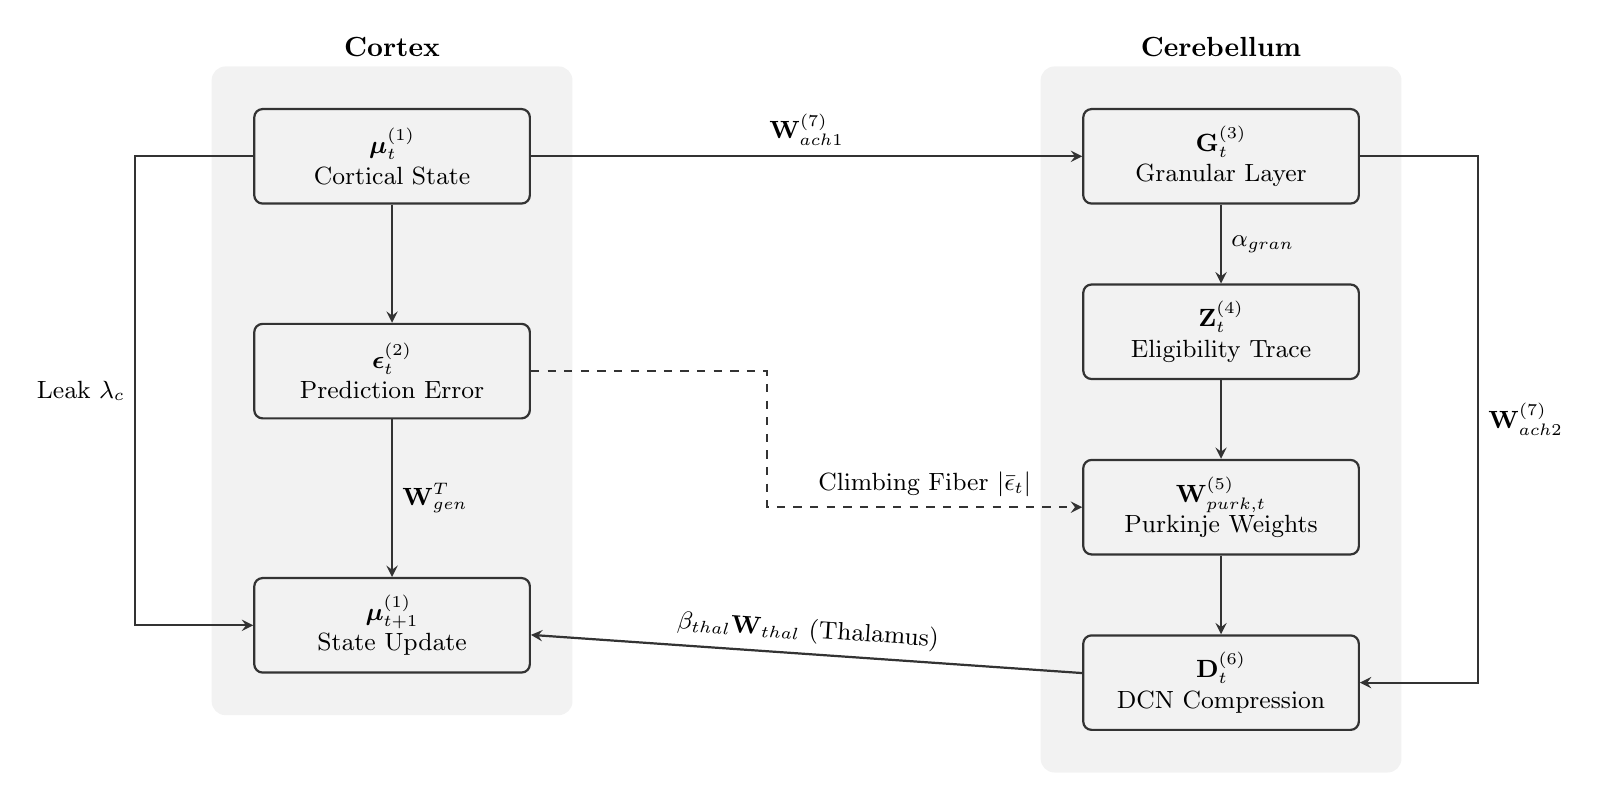
\begin{tikzpicture}[
    >=stealth,
    node distance=1.2cm and 7cm,
    font=\small,
    box/.style={rectangle, draw=black!80, thick, rounded corners=3pt, minimum width=3.5cm, minimum height=1.2cm, align=center},
    module/.style={rectangle, draw=none, fill=gray!10, rounded corners=5pt, inner sep=15pt},
    arrow/.style={->, thick, draw=black!80},
    dasharrow/.style={->, dashed, thick, draw=black!80},
]

% Cortex
\node[box] (mu) {$\boldsymbol{\mu}_t^{(1)}$ \\ Cortical State};
\node[box, below=1.5cm of mu] (error) {$\boldsymbol{\epsilon}_t^{(2)}$ \\ Prediction Error};
\node[box, below=2cm of error] (mu_next) {$\boldsymbol{\mu}_{t+1}^{(1)}$ \\ State Update};

% Cerebellum
\node[box, right=7cm of mu] (gran) {$\mathbf{G}_t^{(3)}$ \\ Granular Layer};
\node[box, below=1cm of gran] (trace) {$\mathbf{Z}_t^{(4)}$ \\ Eligibility Trace};
\node[box, below=1cm of trace] (purk) {$\mathbf{W}_{purk,t}^{(5)}$ \\ Purkinje Weights};
\node[box, below=1cm of purk] (dcn) {$\mathbf{D}_t^{(6)}$ \\ DCN Compression};

% Backgrounds
\begin{scope}[on background layer]
    \node[module, fit=(mu) (error) (mu_next), label={[font=\bfseries]90:Cortex}] (ctx_bg) {};
    \node[module, fit=(gran) (trace) (purk) (dcn), label={[font=\bfseries]90:Cerebellum}] (cer_bg) {};
\end{scope}

% Forward to Cerebellum
\draw[arrow] (mu) -- node[above] {$\mathbf{W}_{ach1}^{(7)}$} (gran);

% Cerebellum internal
\draw[arrow] (gran) -- node[right] {$\alpha_{gran}$} (trace);
\draw[arrow] (trace) -- (purk);
\draw[arrow] (purk) -- (dcn);
\draw[arrow] (gran.east) -- +(1.5,0) |- node[pos=0.25, right] {$\mathbf{W}_{ach2}^{(7)}$} (dcn.east);

% Error to Purkinje
\draw[dasharrow] (error.east) -- +(3.0,0) |- node[pos=0.75, above] {Climbing Fiber $|\bar{\epsilon}_t|$} (purk.west);

% Cortex internal
\draw[arrow] (mu) -- (error);
\draw[arrow] (error) -- node[right] {$\mathbf{W}_{gen}^T$} (mu_next);
\draw[arrow] (mu.west) -- +(-1.5,0) |- node[pos=0.25, left] {Leak $\lambda_c$} (mu_next.west);

% Thalamus return
\draw[arrow] (dcn) -- node[pos=0.5, above, sloped] {$\beta_{thal}\mathbf{W}_{thal}$ (Thalamus)} (mu_next);

\end{tikzpicture}

\vspace{0.5cm}
\begin{minipage}{\linewidth}
\scriptsize
\textbf{(1)} $\boldsymbol{\mu}_{t+1} = \boldsymbol{\mu}_{t} + \alpha_{c} \left[\mathbf{W}^{T}_{gen} \boldsymbol{\epsilon}_{t} - \lambda_{c} ITI_{t} \boldsymbol{\mu}_{t} + \beta_{thal} \mathbf{W}_{thal} \mathbf{D}_{t}\right]$ \\[0.5ex]
\textbf{(2)} $\boldsymbol{\epsilon}_{t} = \Pi \odot (\mathbf{I}_{t} - \hat{\mathbf{I}}_{t})$ \\[0.5ex]
\textbf{(3)} $\mathbf{G}_{t} = \mathbf{W}_{ach1} \boldsymbol{\mu}_{t}$ \\[0.5ex]
\textbf{(4)} $\mathbf{Z}_{t} = (1 - \beta_{gran}) \mathbf{Z}_{t-1} + \alpha_{gran} \mathbf{G}_{t}$ \\[0.5ex]
\textbf{(5)} $\mathbf{W}_{purk, t} = \mathbf{W}_{purk, t-1} - \kappa ( \left| \bar{\epsilon}_{t} \right| \mathbf{Z}_{t})$ \\[0.5ex]
\textbf{(6)} $\mathbf{D}_{t} = \mathbf{W}_{ach2} (\mathbf{G}_{t} \odot \mathbf{W}_{purk, t})$ \\[0.5ex]
\textbf{(7)} $\mathbf{W}_{ach1}, \mathbf{W}_{ach2} \sim \mathcal{N}(0, \sigma_{ach}^2)$
\end{minipage}
\end{center}
\end{document}
